\chapter{User Guide}
Our final application interface is in the form of web and mobile applications for facility the user to choose which is preferred for him. It just requires the user to download the mobile app or browser it. \\

\noindent
This guide is divided into 2 sections:
\begin{itemize}[itemsep=1pt, topsep=5pt]
    \item Web Application
    \item Mobile Application
\end{itemize}

\section{Web Application}
Figure \ref{fig:web-login-page} shows the first page of web application which is login page, the user should login to our app to make use of the full app functionalities. If he didn't have an account, he can simply create one by clicking on \textbf{SingUp} or just can continue as \textbf{Anonymous user} if didn't need to create an account.

\begin{figure}[!htb]
    \centering
    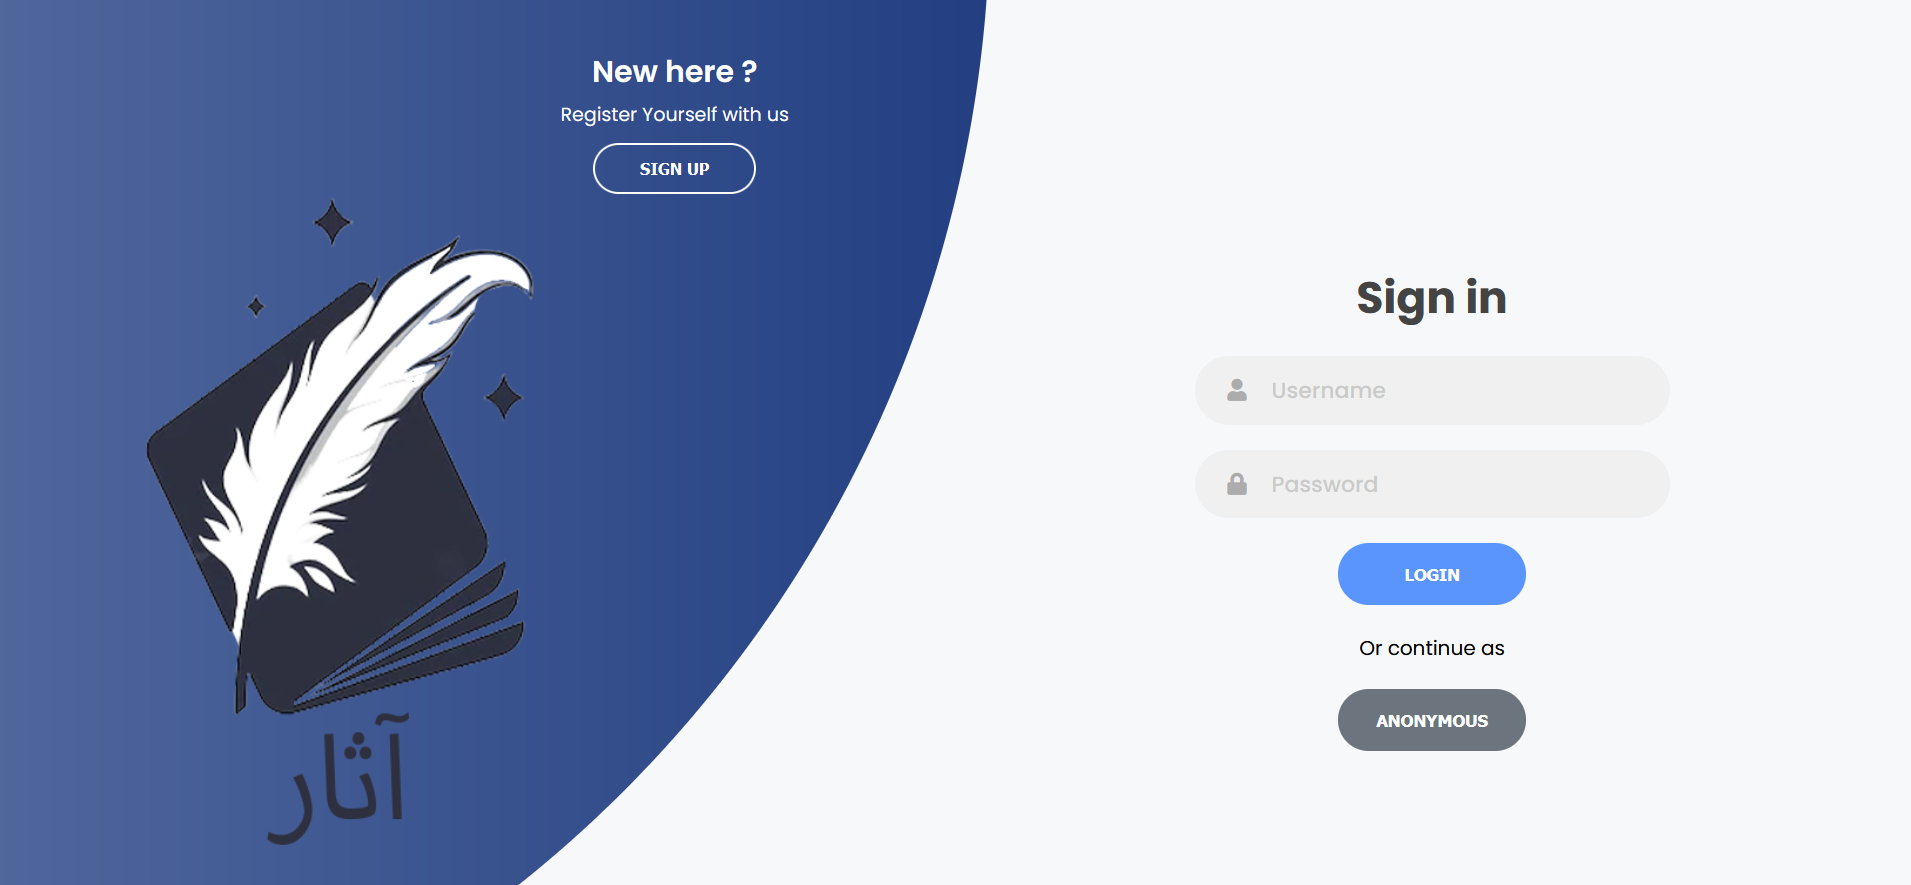
\includegraphics[width=17cm,height=8cm]{images/app/web/web-1.PNG}
    \caption{Login Page of Web Application}
    \label{fig:web-login-page}
\end{figure}

After logging into our app, he will redirect to home page which contains the previous classifications as a history to track and save each prediction. Then, he can download the results of that prediction or just delete it.

\begin{figure}[!htb]
    \centering
    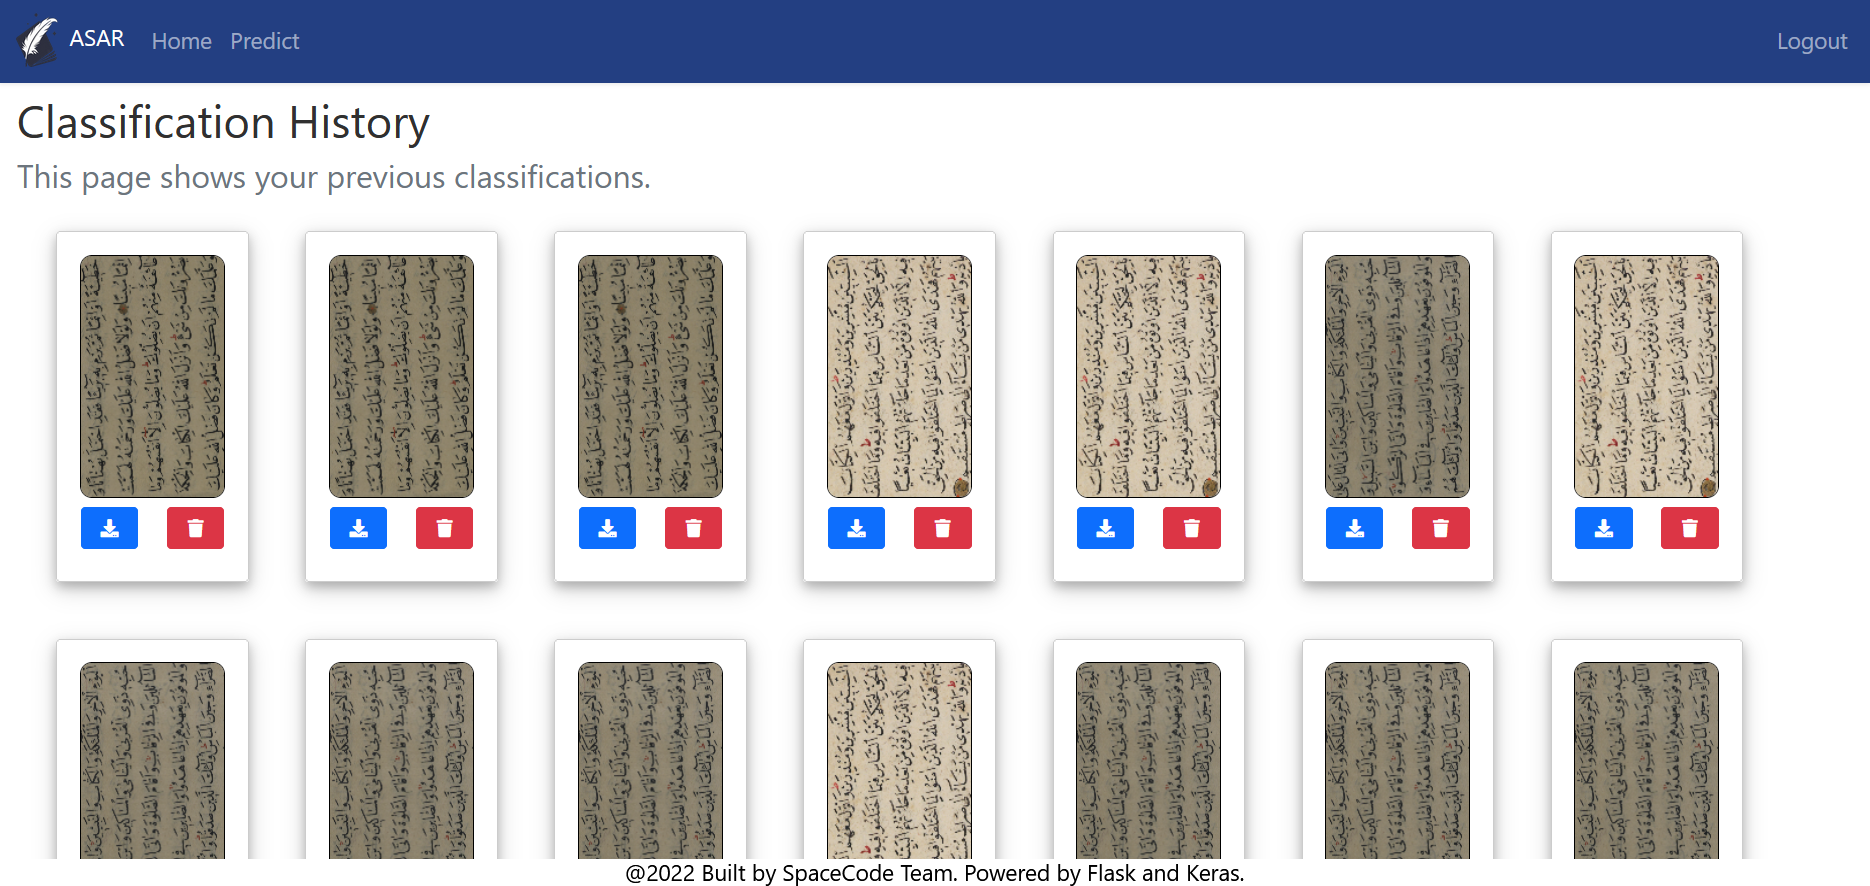
\includegraphics[width=15cm,height=8cm]{images/app/web/web-2.PNG}
    \caption{Home Page of Web Application}
    \label{fig:web-home-page}
\end{figure}

If the user need to digitizing any manuscripts, he will click on Predict tab in the navigation bar, then just upload the image and can crop the image if needed (cropping is necessary for the images have border to focus only the text image)

\begin{figure}[!htb]
    \centering
    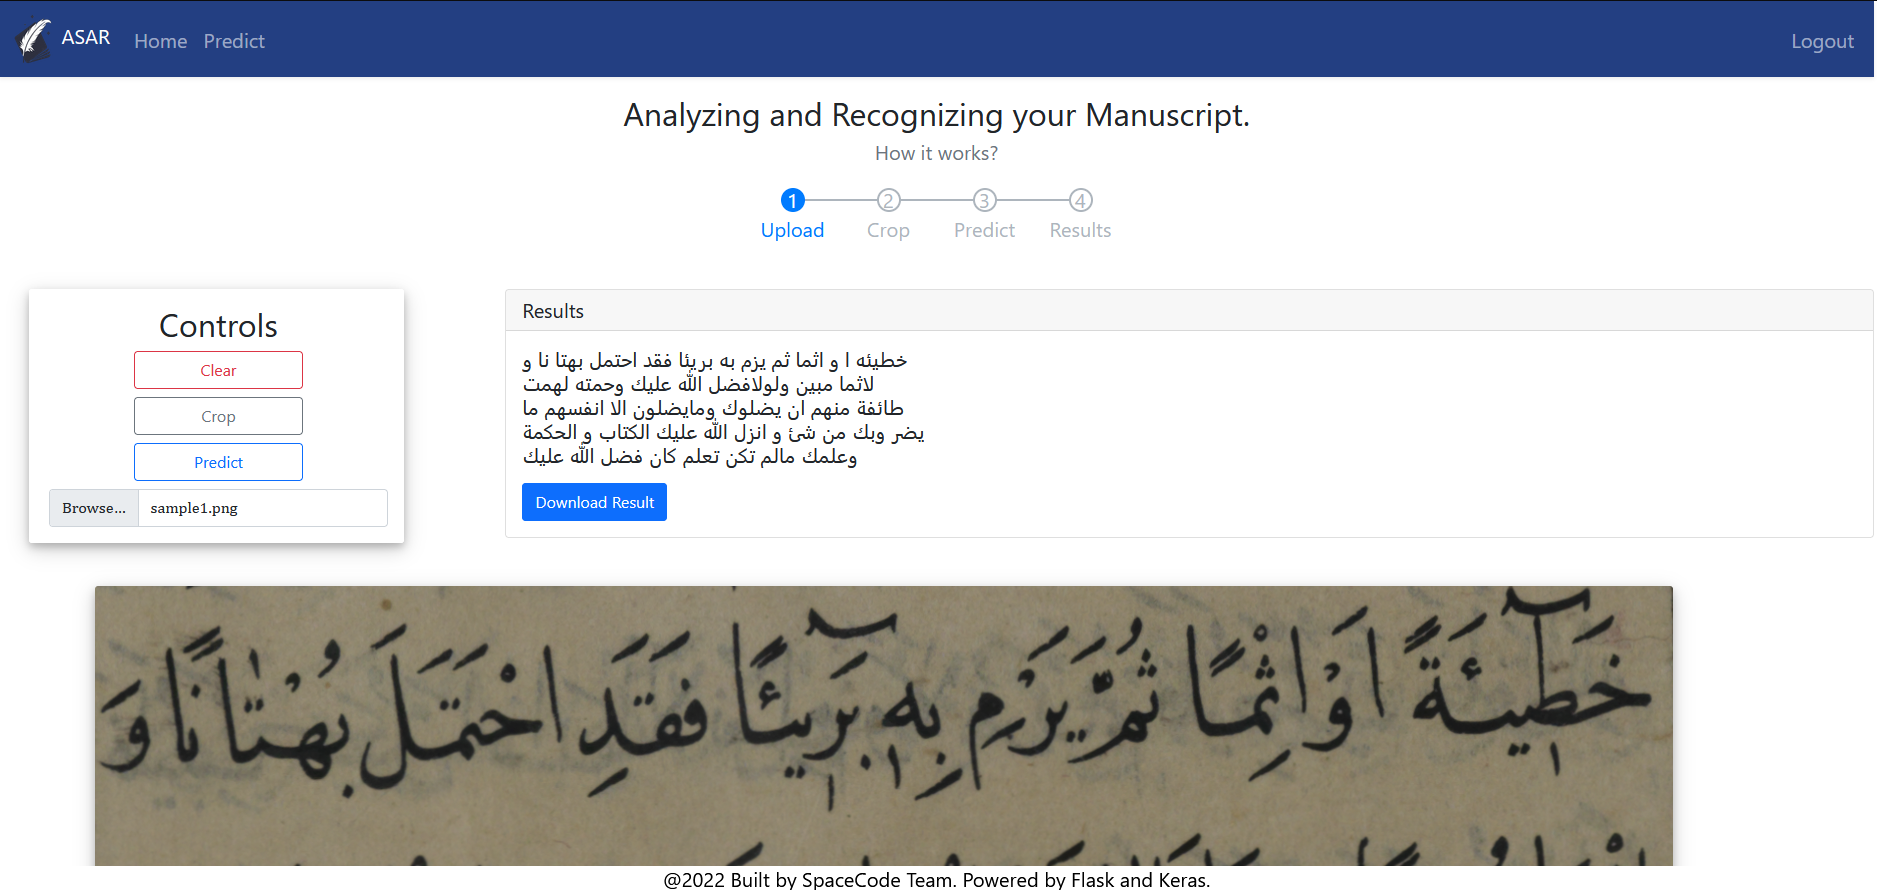
\includegraphics[width=15cm,height=8cm]{images/app/web/web-3.PNG}
    \caption{Home Page of Web Application}
    \label{fig:web-home-page}
\end{figure}

As shown on the figure above, after uploading, and clicks \textbf{Predict}, it will take two minuets to analyzing and recognizing the complete manuscript. Also, you can download the results as text file. \\

Also, in order to connect with Mobile application with the Web application we have build RESTFul \acrshort{api} and used Swagger framework to document API's endpoins to connect with. Figure \ref{fig:web-swagger} shows swagger document screen which you can access it by redirecting the following URL \href{http://127.0.0.1:5000/api/docs}{http://127.0.0.1:5000/api/docs}

\begin{figure}[H]
    \centering
    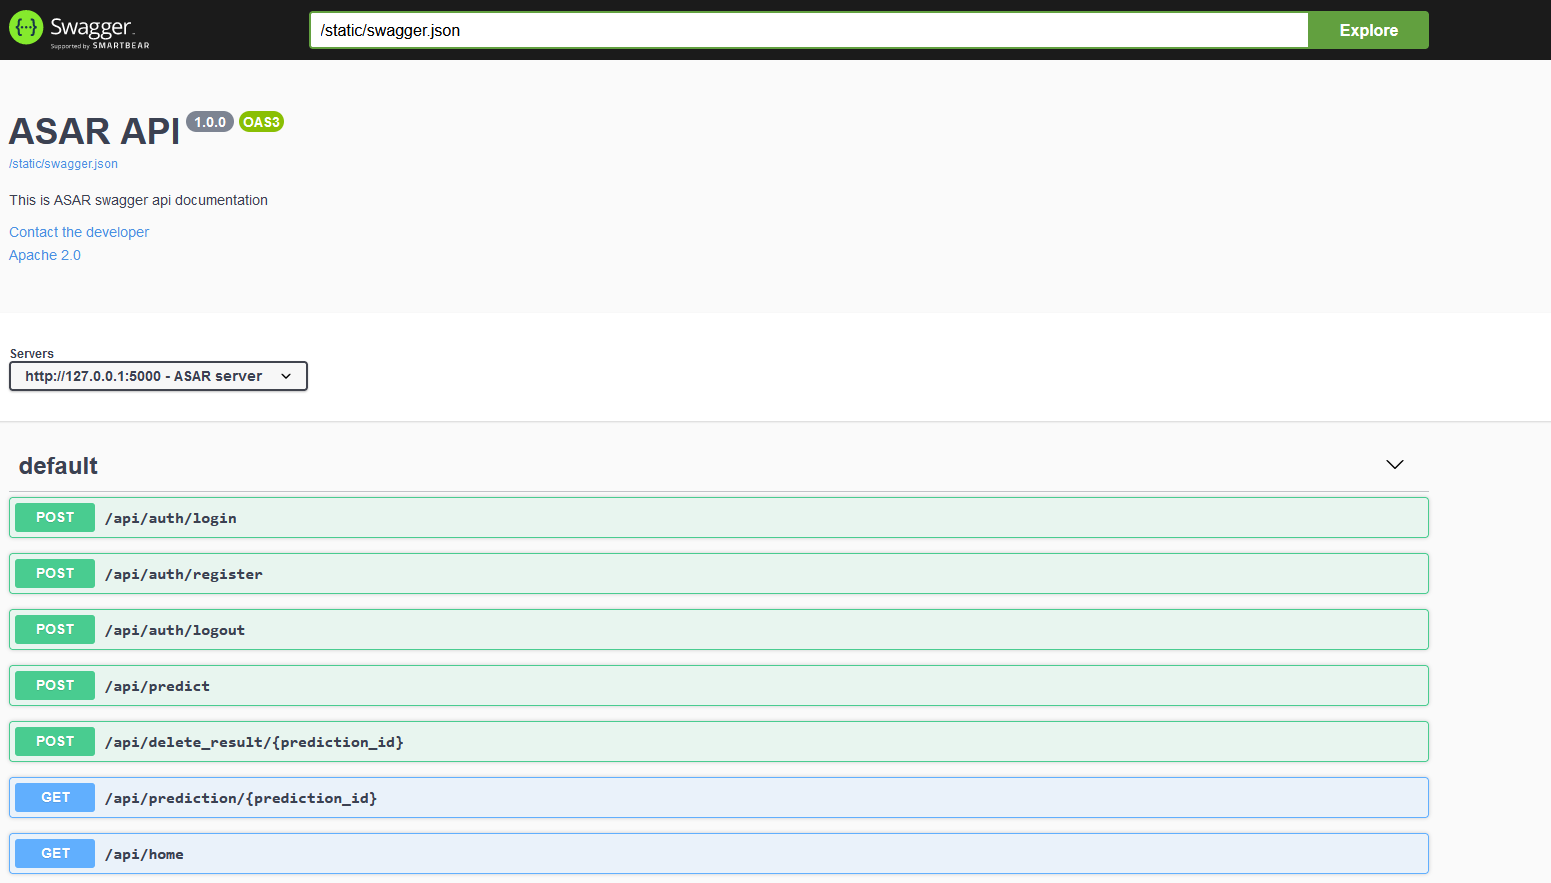
\includegraphics[width=14cm,height=8cm]{images/app/web/web-api-docs.PNG}
    \caption{Swagger API Documentation Page}
    \label{fig:web-swagger}
\end{figure}

\clearpage

\section{Mobile Application}

The flow of the mobile application will be the same as mention in the web application section. The following list of figures shows the mobile app flow in order to digitize your historical manuscript.

\begin{figure}[H]
     \centering%
     \begin{subfigure}[b]{0.3\textwidth}
         \centering
         
\includegraphics[width=\textwidth]{images/app/mobile/mobile-1.png}
         \caption{Login Screen}
         \label{fig:mobile-login-screen}
     \end{subfigure}
     \hfill
      \begin{subfigure}[b]{0.3\textwidth}
         \centering
         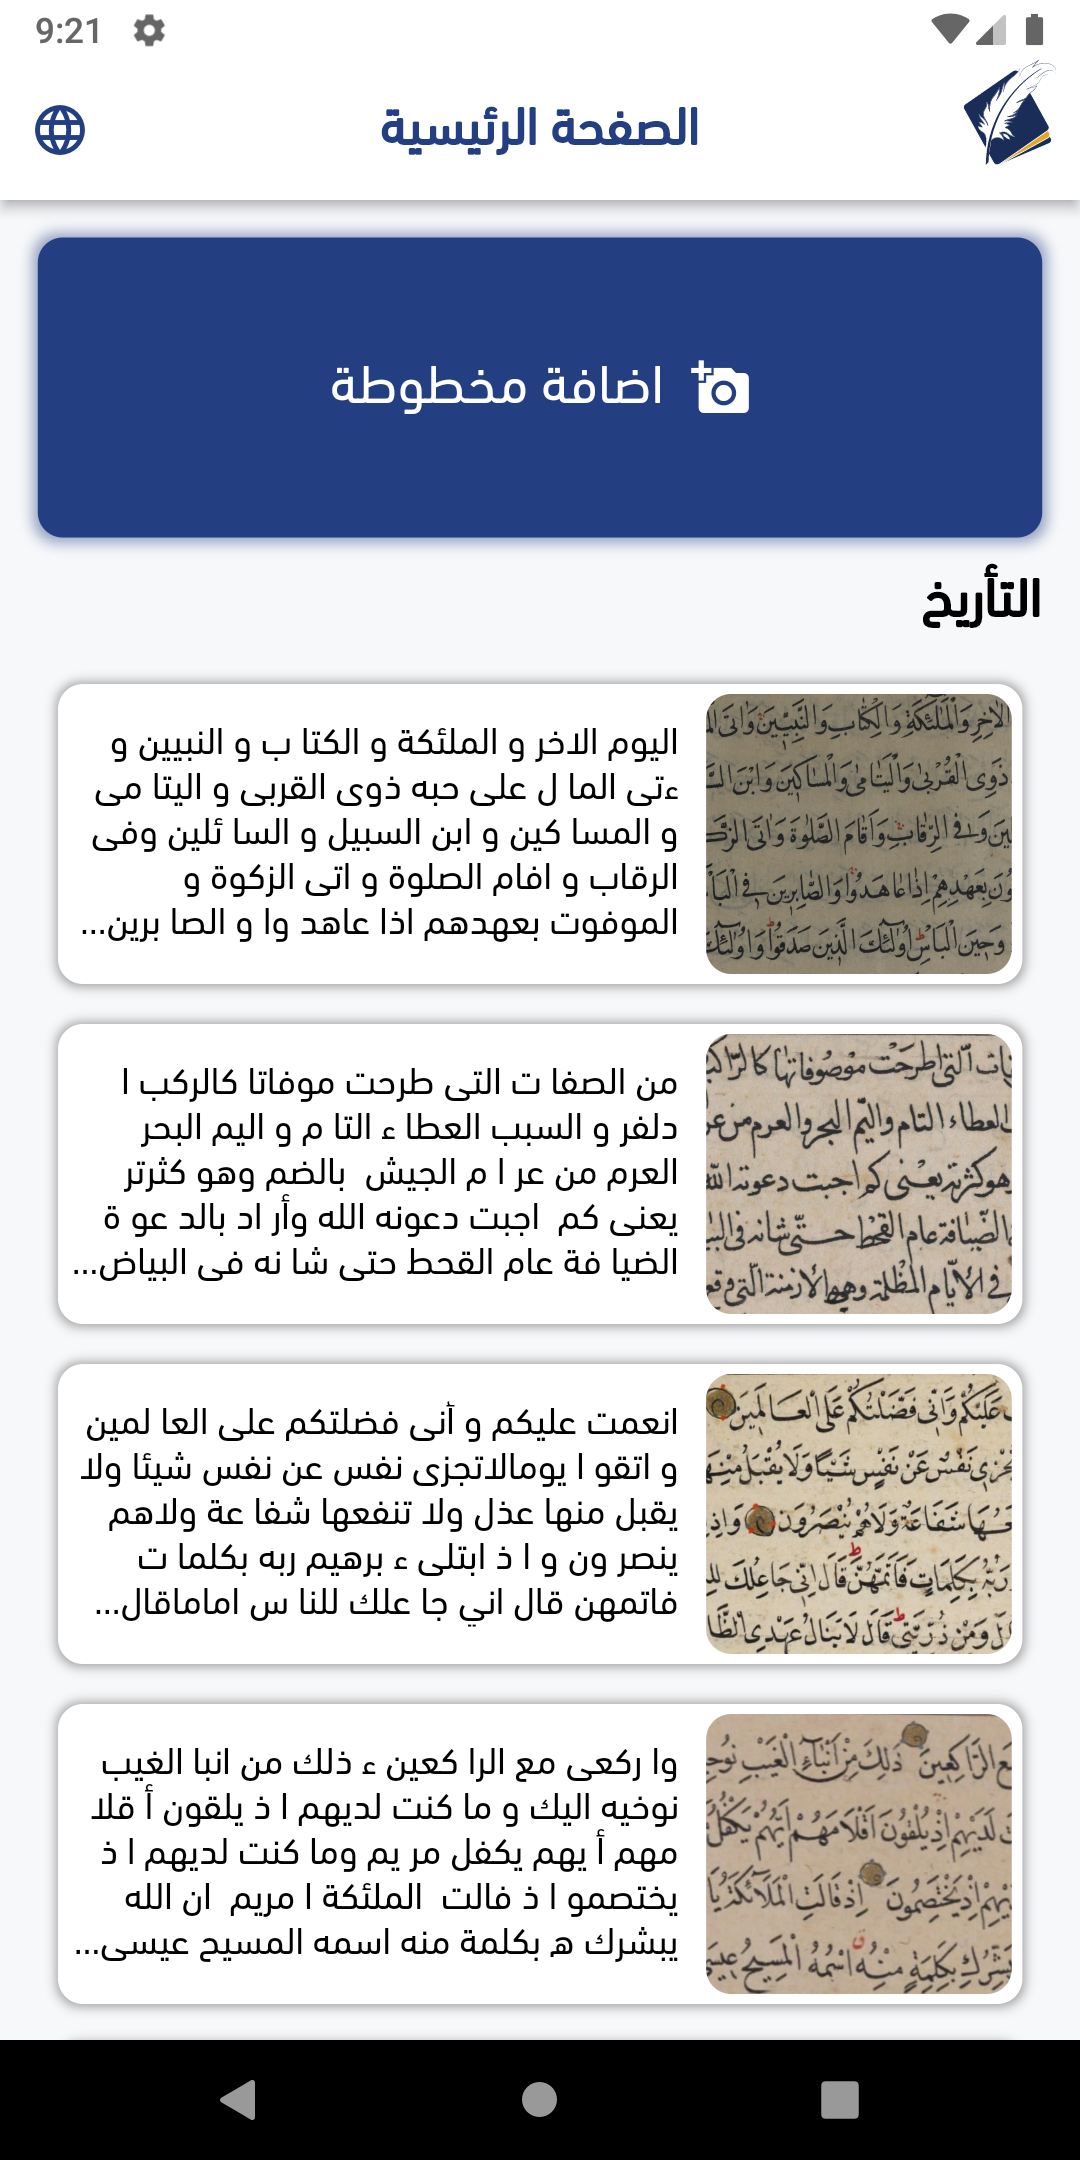
\includegraphics[width=\textwidth]{images/app/mobile/mobile-2.png}
         \caption{Home Screen}
         \label{fig:mobile-home-screen}
     \end{subfigure}
     \hfill%
      \begin{subfigure}[b]{0.3\textwidth}
         \centering
         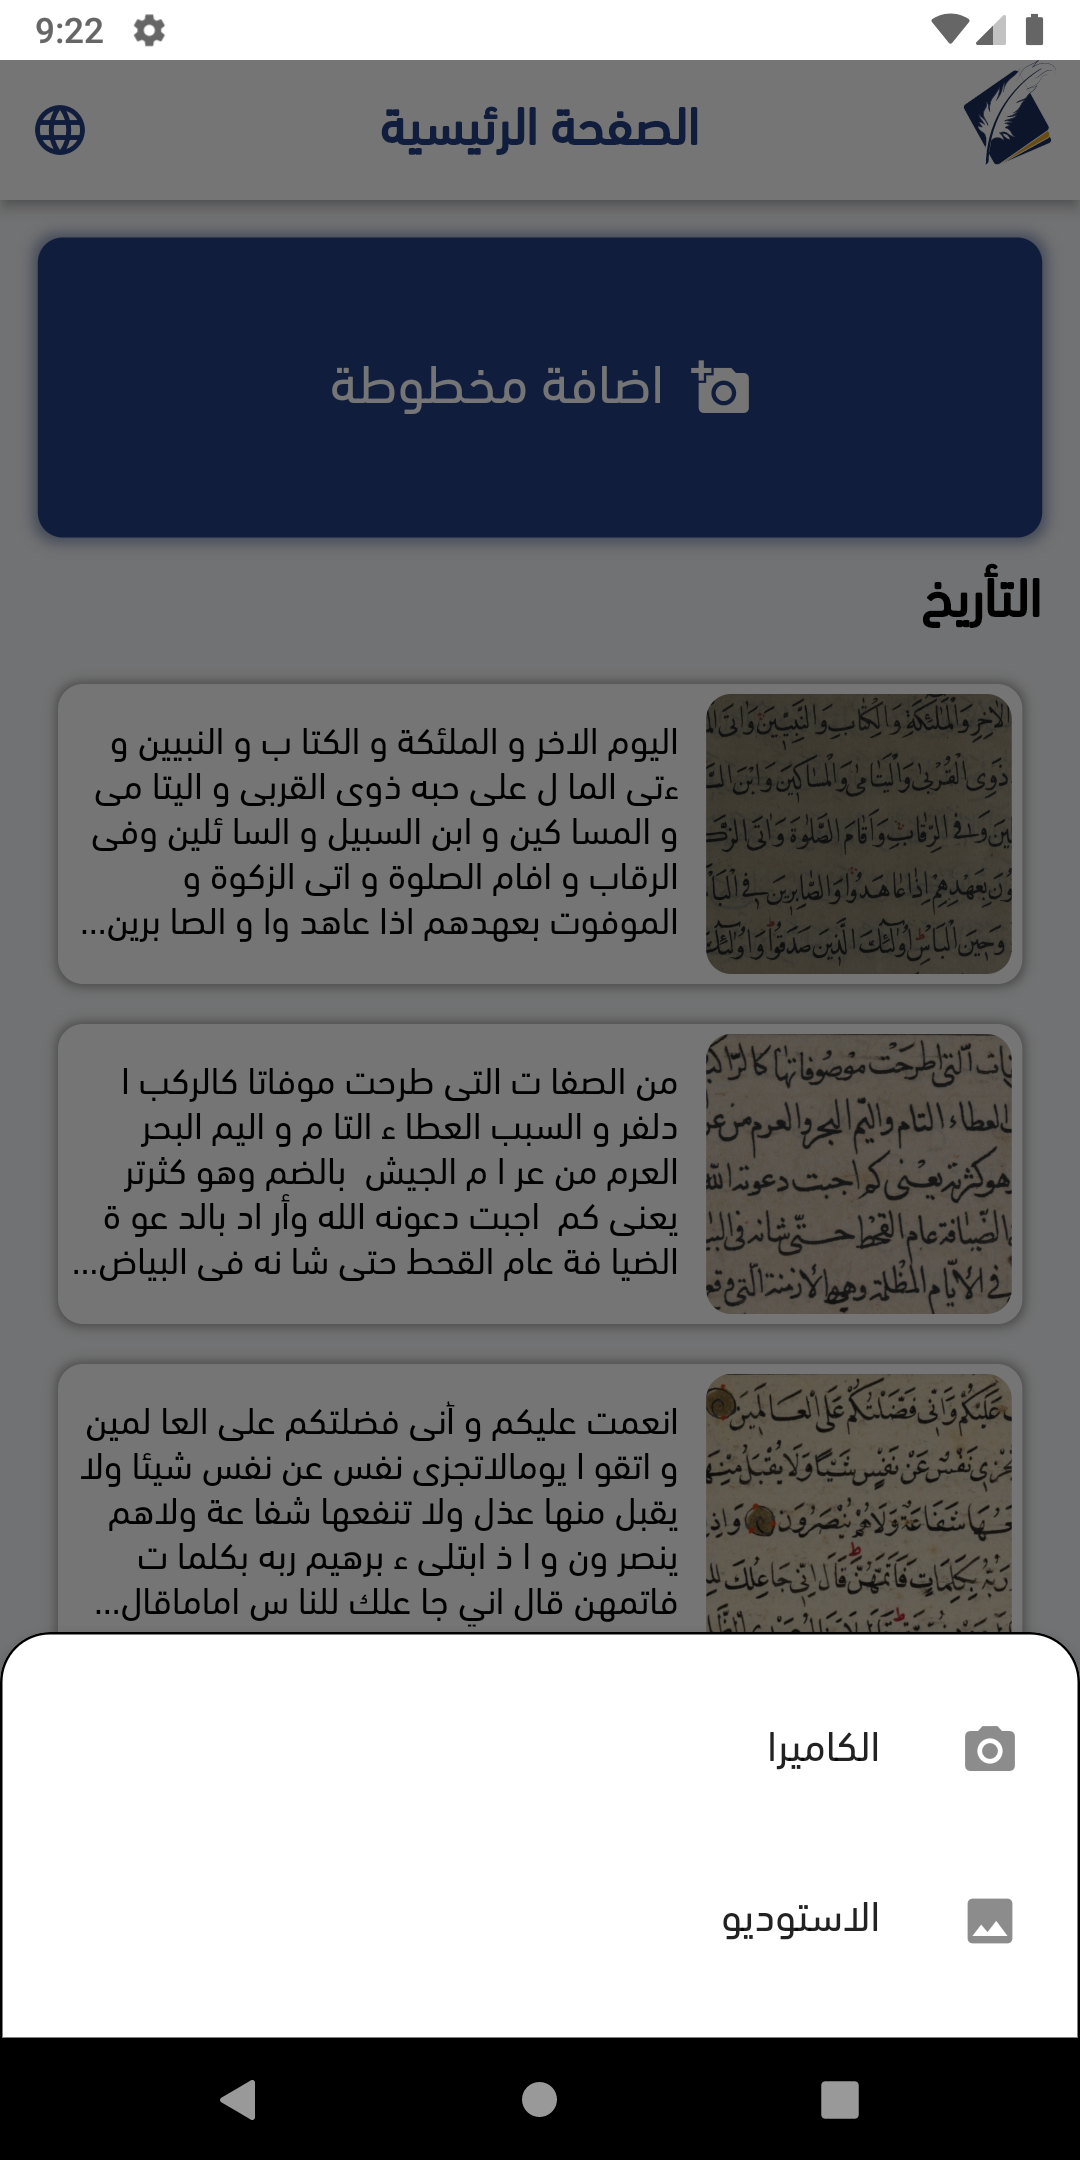
\includegraphics[width=\textwidth]{images/app/mobile/mobile-3.png}
         \caption{Select Image Screen}
         \label{fig:mobile-select-image}
     \end{subfigure}
      \begin{subfigure}[b]{0.3\textwidth}
         \centering
         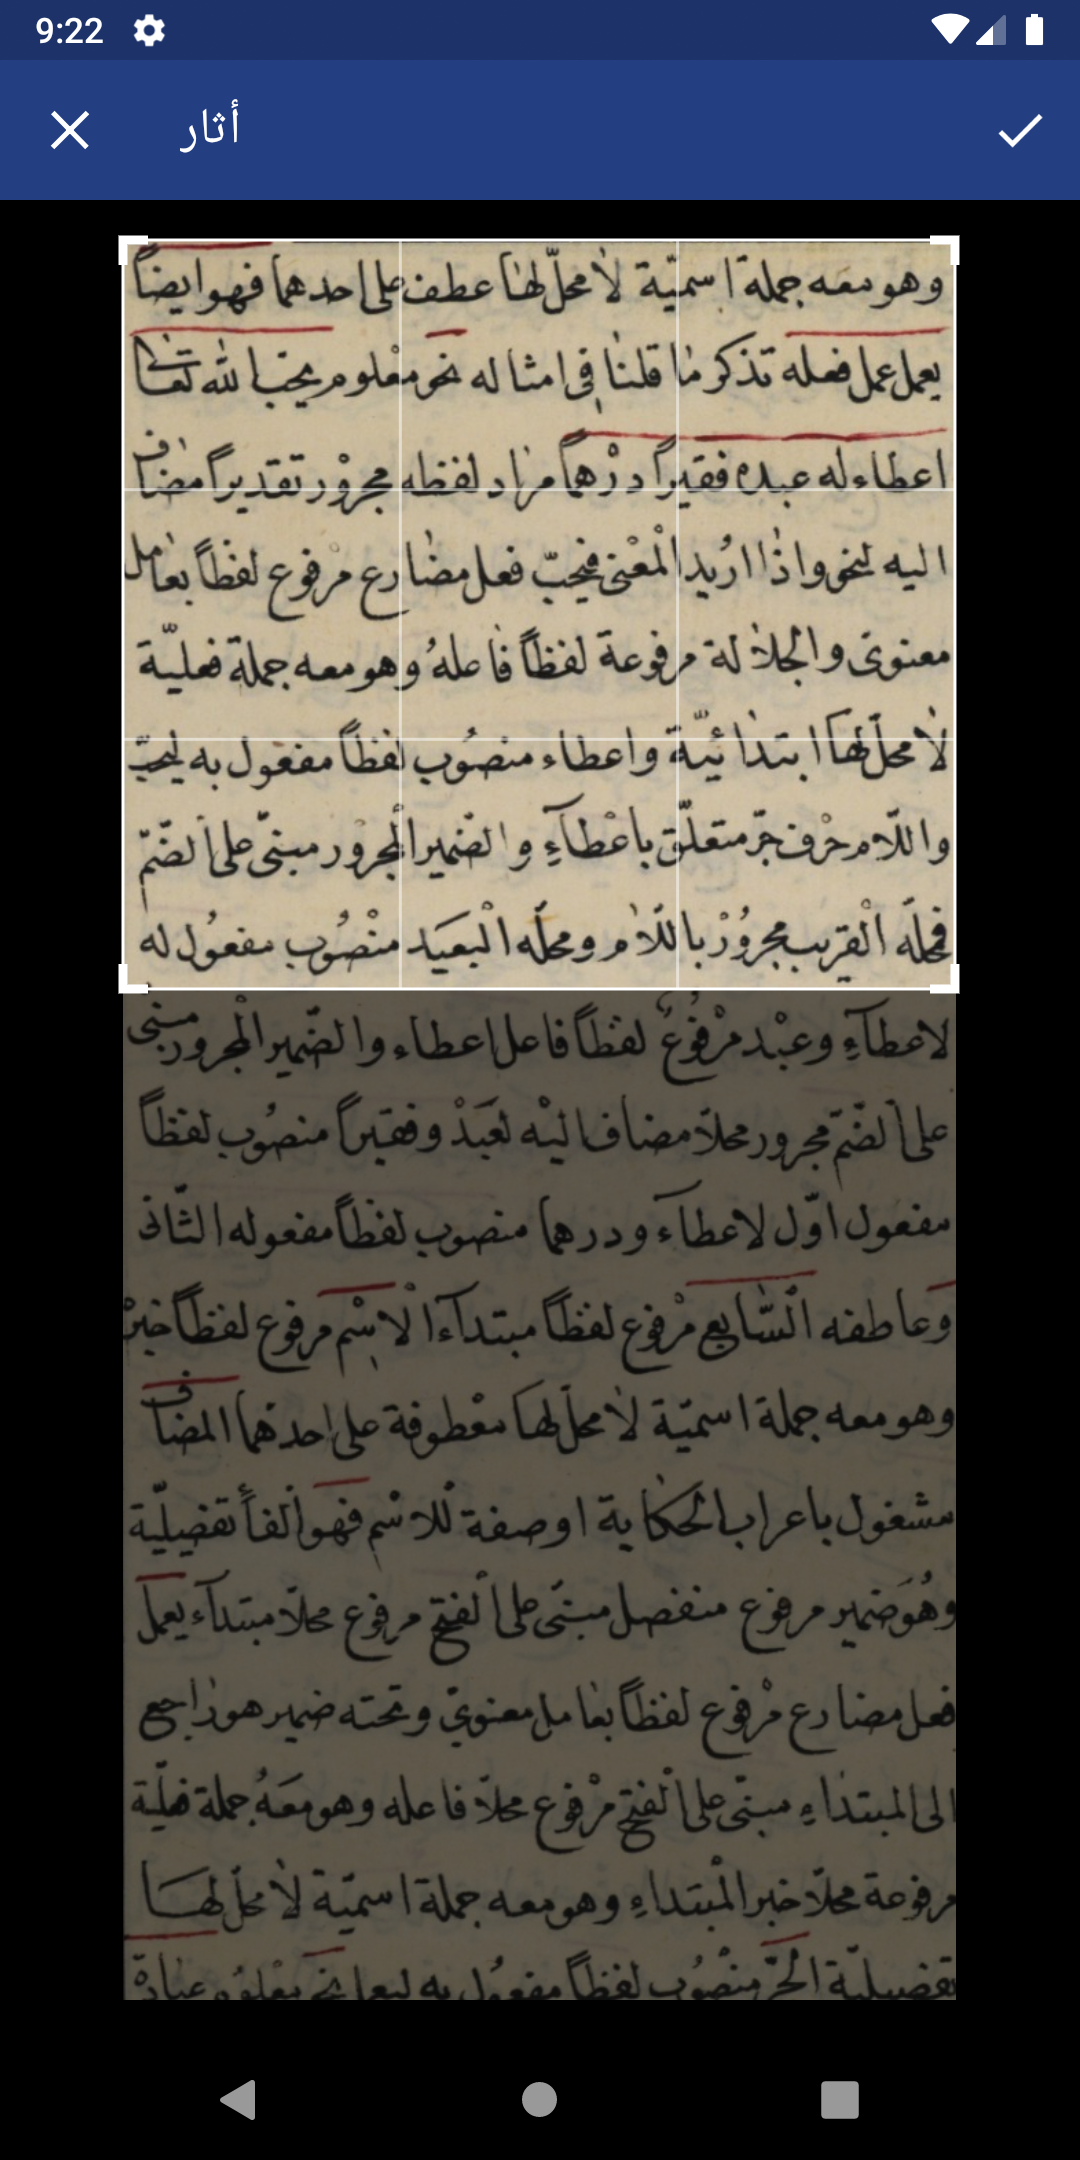
\includegraphics[width=\textwidth]{images/app/mobile/mobile-4.png}
         \caption{Crop Image Screen}
         \label{fig:mobile-crop-image}
     \end{subfigure}
     \hspace{1cm}
      \begin{subfigure}[b]{0.3\textwidth}
         \centering
         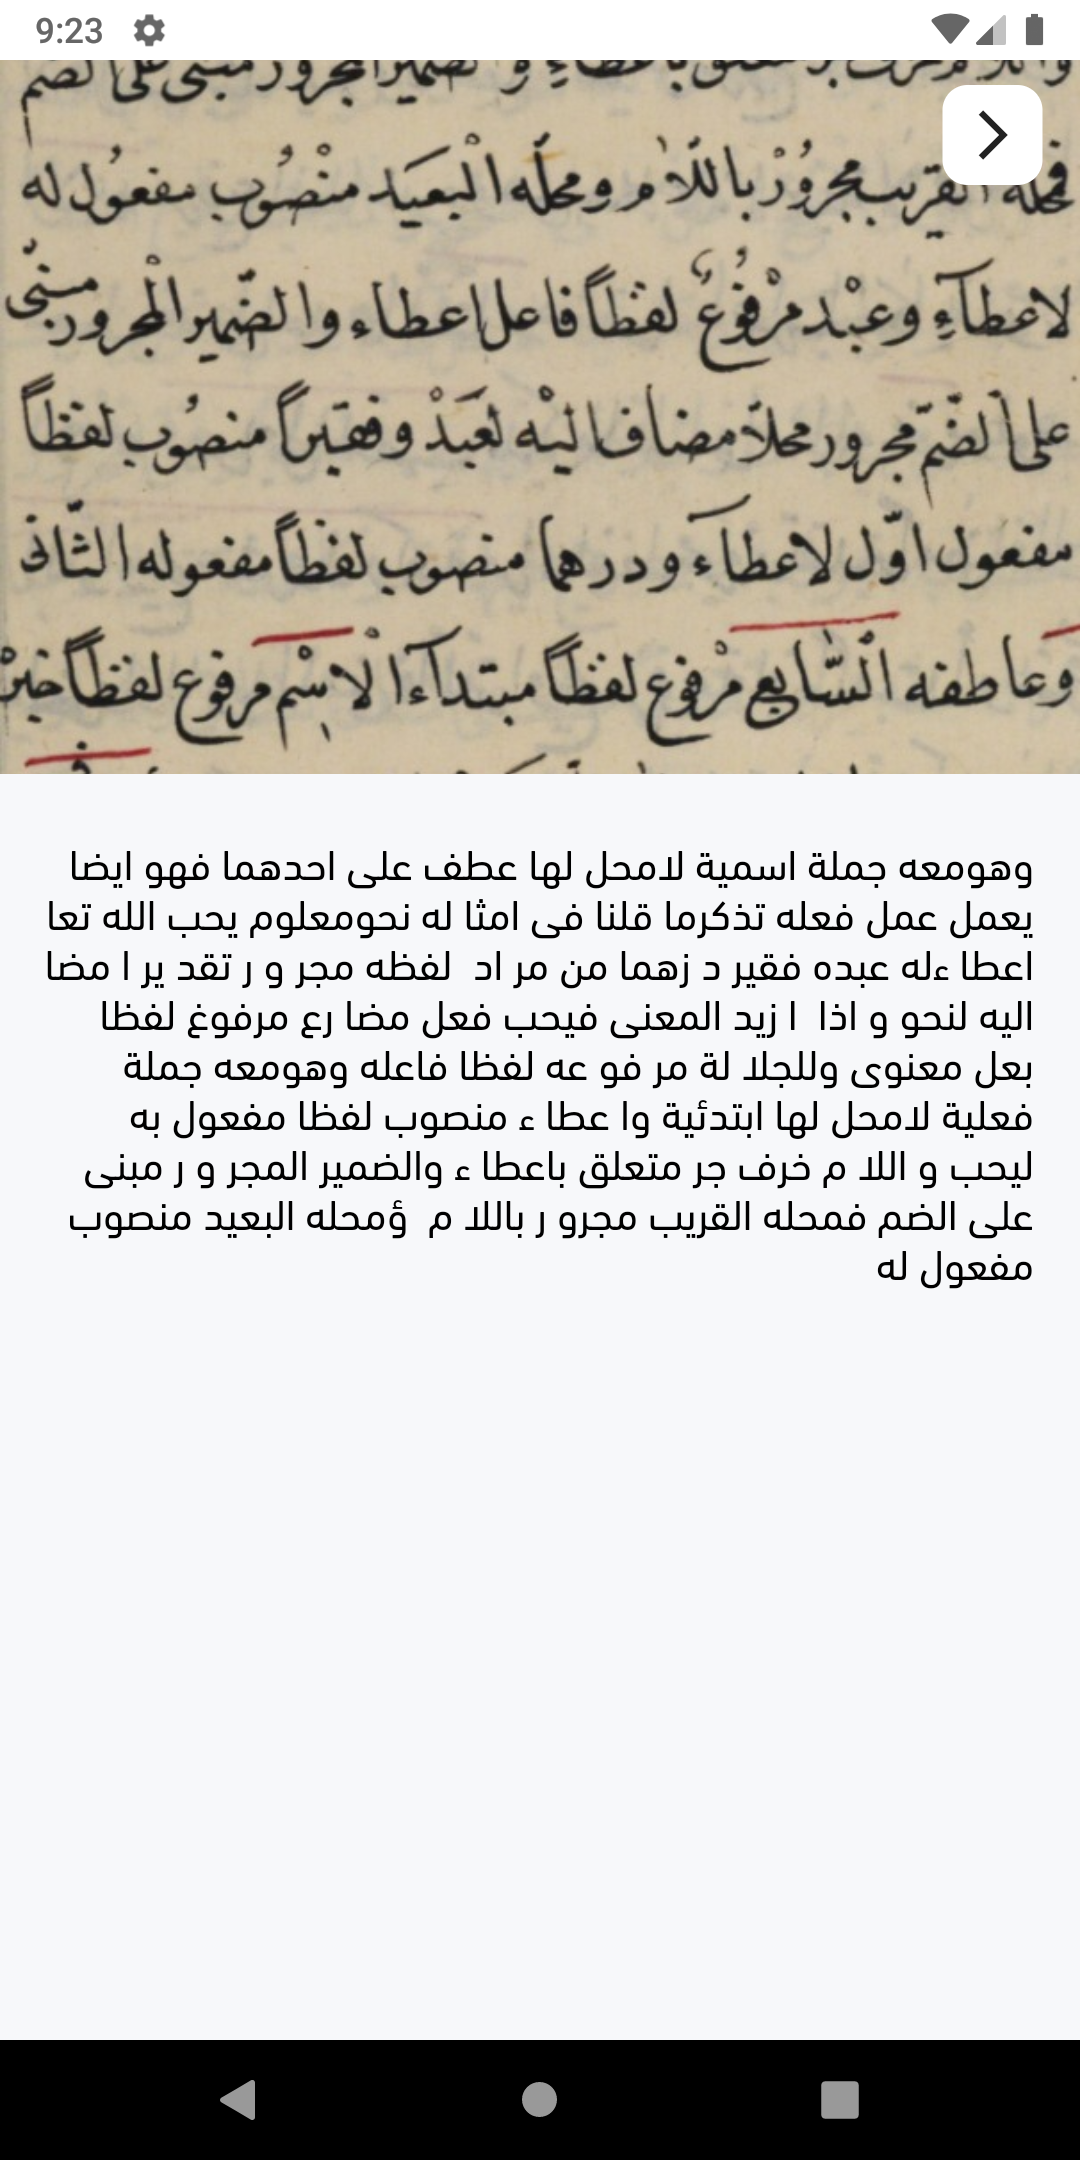
\includegraphics[width=\textwidth]{images/app/mobile/mobile-5.png}
         \caption{Results Screen}
         \label{fig:mobile-results-screen}
     \end{subfigure}
    \caption{Mobile Application Screens.}
    \label{fig:mobile-app-screens}
\end{figure}
